% Generated by pysimcount.pffigure -- do not edit; regenerate instead.
% figure: B-order4-by-formula -- Every order-4 formula at measured r
% source: results/np-main/seed1/results.json
% metric=t gatebase=ct merged
% seed=1 t=n template=simcount synth=pygridsynth
% git_commit=01d3c275ceae2840002bd1aaea68f59b987c4975 git_dirty=False
% source_sha256=0dd1c9775f148df550d3d3f68cfeee1d2d060b7913324535bbf1533b52b4d2c2
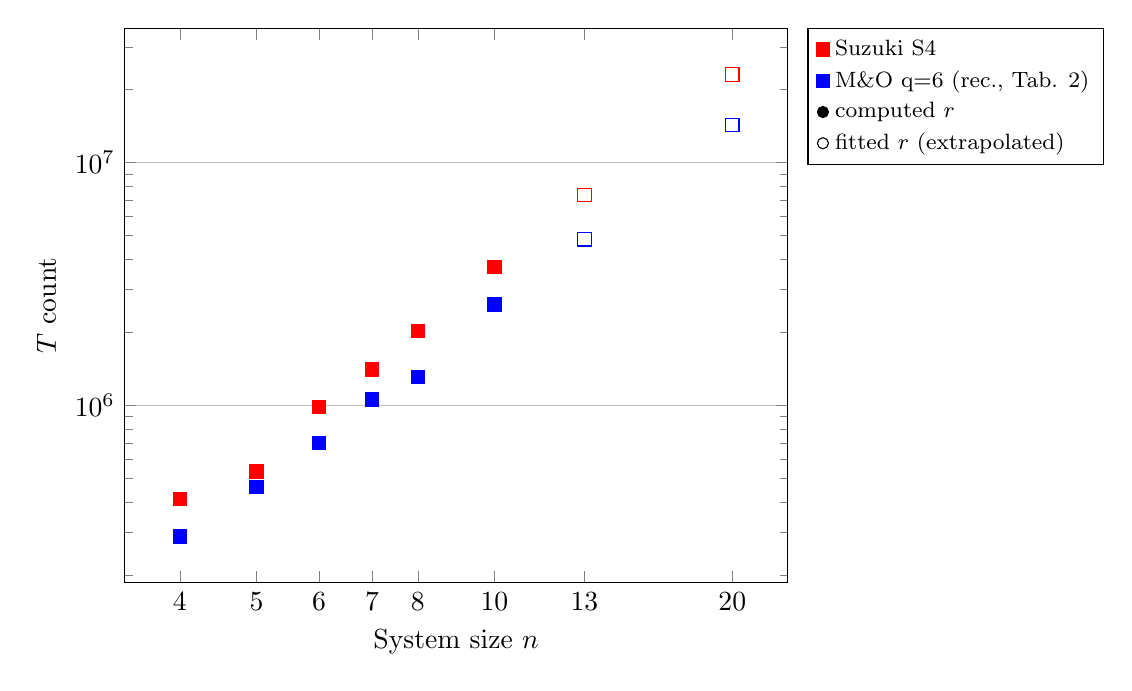
\begin{tikzpicture}
  \begin{loglogaxis}[
    width=10cm,
    xlabel={System size $n$},
    ylabel={$T$ count},
    xtick={4,5,6,7,8,10,13,20},
    xticklabels={4,5,6,7,8,10,13,20},
    ymajorgrids=true,
    legend pos=outer north east,
    legend cell align=left,
    legend style={font=\footnotesize},
  ]
    \addplot[only marks, red, mark=square*, mark size=2.4pt, mark options={solid, fill=red}] coordinates {
      (4,410856)
      (5,534710)
      (6,987026)
      (7,1404340)
      (8,2020560)
      (10,3710728)
    };
    \addlegendentry{Suzuki S4}
    % r from power-law fit (extrapolation); one legend entry per series
    \addplot[only marks, red, mark=square*, mark size=2.4pt, mark options={solid, fill=white}, forget plot] coordinates {
      (13,7377150)
      (20,23100384)
    };
    \addplot[only marks, blue, mark=square*, mark size=2.4pt, mark options={solid, fill=blue}] coordinates {
      (4,288000)
      (5,461360)
      (6,701600)
      (7,1058148)
      (8,1310224)
      (10,2607488)
    };
    \addlegendentry{M\&O q=6 (rec., Tab. 2)}
    % r from power-law fit (extrapolation); one legend entry per series
    \addplot[only marks, blue, mark=square*, mark size=2.4pt, mark options={solid, fill=white}, forget plot] coordinates {
      (13,4833430)
      (20,14317248)
    };
    \addlegendimage{only marks, black, mark=*, mark options={fill=black}}
    \addlegendentry{computed $r$}
    \addlegendimage{only marks, black, mark=*, mark options={fill=white}}
    \addlegendentry{fitted $r$ (extrapolated)}
  \end{loglogaxis}
\end{tikzpicture}
